\renewcommand{\theequation}{\theenumi}
\renewcommand{\thefigure}{\theenumi}
\begin{enumerate}[label=\thesubsection.\arabic*.,ref=\thesubsection.\theenumi]
\numberwithin{equation}{enumi}
\numberwithin{figure}{enumi}

\item Find the distance between the following pair of points
(11,16) and (23,21).\\
Let 
\begin{align}
    \vec{A} = \myvec{11\\16}, \vec{B} = \myvec{23\\21}
\end{align}
Then,
\begin{align}
\vec{B}-\vec{A} = \myvec{12\\5}\;
\end{align}
and
%
\begin{align}
 \norm{\vec{B}-\vec{A}}^2= (\vec{B}-\vec{A})^\top (\vec{B}-\vec{A})\;
&=  \myvec{12 \ 5} \myvec{12\\5}\\
\implies \norm{\vec{B}-\vec{A}}&=\sqrt{(12^2 + 5^2)}\\\nonumber
&=13\\\nonumber
\end{align}



\item Find the distance between the following pair of points
(66,25) and (99,69).
\\
Let
\begin{align}
    \vec{A} = \myvec{66\\25}, \vec{B} = \myvec{99\\69}
\end{align}
Then
\begin{align}
\norm{\vec{B}-\vec{A}}=\norm{\vec {C}}
\end{align}
\begin{align}
 \norm{\vec{C}}^2 &= \vec{C}^\top \vec{C} \\
&=  \myvec{33 \ 44} \myvec{33\\44}\\
\implies \norm{\vec{C}}=\sqrt{(33^2 + 44^2)}\\
&=55
\end{align}
%
\item Find the distance between the following pairs of points  with the axes at 60\degree
\begin{enumerate}
    \item \myvec{7\\6} and \myvec{4\\5}
    \solution{2/solution/2/1/Assignment1.tex}
\end{enumerate}
\item Find the area of the quadrilateral formed by the points
\begin{enumerate}
\item 
\begin{align}
\begin{split}
\vec{A} = \myvec{1 \\ 1}, 
\vec{B} = \myvec{3 \\ 5}, 
\vec{C} = \myvec{-2 \\ 4}, 
\vec{D} = \myvec{-1 \\ -5}.
\end{split}
\end{align}
\solution
Let 
\begin{align}
\begin{split}
\vec{A} = \myvec{1 \\ 1}, 
\vec{B} = \myvec{3 \\ 5}, 
\vec{C} = \myvec{-2 \\ 4}, 
\vec{D} = \myvec{-1 \\ -5}. 
\end{split}
\end{align}
Then, 
\begin{align}
\brak{\vec{B} - \vec{A}}
    &= \myvec{3\\5} - \myvec{1\\1}
    = \myvec{2\\4}
\\
    \brak{\vec{D} - \vec{B}}
    &= \myvec{-1\\-5} - \myvec{3\\5}
    = \myvec{-4\\-10}
\\
     \brak{\vec{A} - \vec{D}}
    &= \myvec{1\\1} - \myvec{-1\\-5}
    = \myvec{2\\6}
\end{align}
%
Row reducing the matrix formed by the  vectors, 
\begin{align}
%\begin{math}
\myvec{2 & 4 & 1\\-4 & -10 & 1\\2 & 6 & 1\\}
\\
\implies 
\myvec{2 & 4 & 1\\-4 & -10 & 1\\2 & 6 & 1\\}
\xleftrightarrow[]{R_2\leftrightarrow R_3}
\myvec{2 & 4 & 1\\2 & 6 & 1\\-4 & -10 & 1\\}
\xleftrightarrow[]{R_3\leftrightarrow R_1+R_2+R_3}
\myvec{2 & 4 & 1\\2 & 6 & 1\\0 & 0 & 3\\}
\xleftrightarrow[]{R_2\leftrightarrow R_2-R_1}
\myvec{2 & 4 & 1\\0 & 2 & 0\\0 & 0 & 3\\}
%\end{math}
\end{align}
The number of non-zero rows in the matrix = 3. Hence the matrix
is full rank and  AB, BD, DA are not collinear.
See Fig. \ref{hem/2/9/1/fig:Quad ABCD}, which shows that the points given form a quadrilateral.
\begin{figure}[!ht]
    \centering
    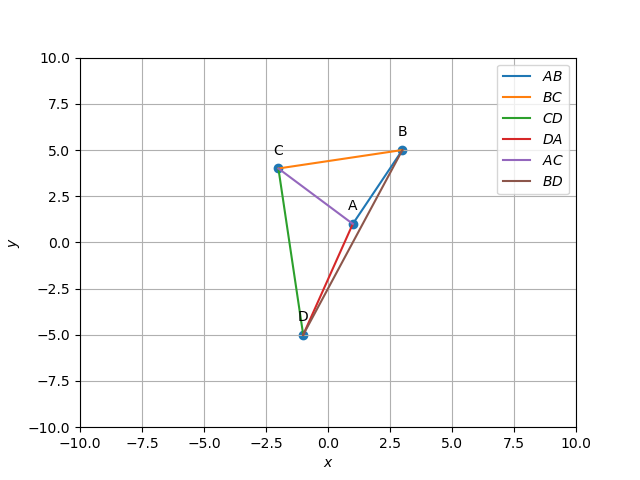
\includegraphics[width=\columnwidth]{2/solution/9/1/QUAD.png}
    \caption{Quadrilateral ABCD}
    \label{hem/2/9/1/fig:Quad ABCD}
\end{figure}
%
Area of a $\triangle ABC$ is given by
%
\begin{align}
\triangle ABC = 
\frac{1}{2}\mydet{
1 & 1 & 1\\1 & 3 & -2\\1 & 5 & 4\\}
= 9
\end{align}
%
Area of $\triangle ACD$  is given by
\begin{align}
\triangle ACD = 
\frac{1}{2}\mydet{
1 & 1 & 1\\1 & -2 & -1\\1 & 4 & -5\\}
= 11.5
\end{align}
Thus, the area of quadrilateral ABCD = 9+11.5 = 20.5.

\item 
\begin{align}
\vec{P} = \myvec{2\\1}, \vec{Q} =\myvec{3\\5},
\vec{R} =\myvec{-3\\4}, \vec{S} =\myvec{-2\\-2}
\end{align}
\solution

In Fig.     \ref{2/9/2fig:Quad PQRS},
 Area of a Quadrilateral PQRS=
\begin{align}
Area (\triangle PQR)+ Area (\triangle PRS)=
\end{align}
\begin{equation}
\frac{1}{2}\norm{(\vec{Q}-\vec{P})\times(\vec{Q}-\vec{R})}+\frac{1}{2}\norm{\mathbf{(\vec{S}-\vec{P})\times(\vec{S}-\vec{R})}}
\label{2/9/2eq:1}
\end{equation}
For two vectors
\begin{align}
\vec{a}=\myvec{a_1\\a_2} , \vec{b}=\myvec{b_1\\b_2}
\end{align}
\begin{equation}
\norm{\mathbf{\vec{a}\times\vec{b}}}=\abs{(a_1b_2-a_2b_1)}
\label{2/9/2eq:2}
\end{equation}
\begin{align}
\vec{Q-P}=\myvec{1\\4}\\
\vec{Q-R}=\myvec{6\\1}\\
\vec{S-P}=\myvec{-4\\-3}\\
\vec{S-R}=\myvec{1\\-6}
\end{align}
Using equation \eqref{2/9/2eq:2}
\begin{equation}
\frac{1}{2}\norm{\mathbf{(\vec{Q}-\vec{P})\times(\vec{Q}-\vec{R})}}
=\frac{1}{2}\abs{(-23)}=11.5
\label{2/9/2eq:3}
\end{equation}
\begin{equation}
\frac{1}{2}\norm{\mathbf{(\vec{S}-\vec{P})\times(\vec{S}-\vec{R})}}
=\frac{1}{2}\abs{(27)}=13.5    
\label{2/9/2eq:4}
\end{equation}
Substituting values from equation \eqref{2/9/2eq:3} and \eqref{2/9/2eq:4} in equation \eqref{2/9/2eq:1},the desired area is
\begin{align}
11.5+13.5
=25 
\end{align}
\begin{figure}[!ht]
    \centering
    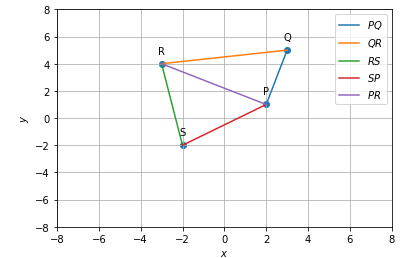
\includegraphics[width=\columnwidth]{2/solution/2/9/2/QUAD.PNG}
    \caption{Quadrilateral PQRS}
    \label{2/9/2fig:Quad PQRS}
\end{figure}




\end{enumerate}
\end{enumerate}
